\documentclass[11pt, a4paper, spanish]{article}
     
\usepackage{float}
\usepackage{wrapfig}
\usepackage{sidecap}
\usepackage{subcaption}
\usepackage[a4paper, margin=2.5cm, top=3.5cm, bottom=3.5cm]{geometry} % Define los márgenes
\usepackage{amsmath, amscd, amssymb, amsthm, latexsym, gensymb} % Paquetes matemáticos
\usepackage[spanish]{babel} % Traduce los paquetes a español
\usepackage{ dsfont } %para usar simbolo de Naturales
\usepackage[utf8]{inputenc} % Codificación UTF8
\usepackage{fancyhdr} % Encabezados y pies de página
    \pagestyle{fancyplain}
\usepackage{enumerate}
\usepackage{xspace}
%\usepackage[page, toc]{appendix} % Apéndices
%\usepackage[nottoc]{tocbibind} % Referencias en la TDC
\usepackage{scrextend} % Para usar addmargin
\usepackage{listings} % Código
    \lstdefinestyle{customcpp}{
        belowcaptionskip=1\baselineskip,
        breaklines=true,
        xleftmargin=3em,
        language=C++,
        basicstyle=\small\ttfamily
    }
\usepackage[onelanguage, spanish]{algorithm2e}
    % \NoCaptionOfAlgo
    \LinesNumbered\RestyleAlgo{ruled}\IncMargin{1em}\DontPrintSemicolon\SetArgSty{}\SetCommentSty{textsf}\SetFuncSty{textsf}
    \SetKwProg{For}{para}{ hacer}{fin}
    \SetKwProg{Fn}{función}{:}{fin}
\usepackage[pdftex]{graphicx} % Imágenes
\usepackage[usenames,dvipsnames]{color} % Autoexplicativo
\usepackage{caption} % Captions sin números
\usepackage{multirow}
\usepackage{caratula} % Carátula del DC
\usepackage{url}

\usepackage{xspace}
\usepackage{xargs}
\usepackage{ifthen}



\let\NombreFuncion=\textsc
\let\TipoVariable=\texttt
\let\tipo=\texttt
\let\ModificadorArgumento=\textbf
\newcommand{\res}{$res$\xspace}
\newcommand{\tab}{\hspace*{7mm}}


\newcommandx{\TipoFuncion}[3]{%
  \NombreFuncion{#1}(#2) \ifx#3\empty\else $\to$ \res\,: \TipoVariable{#3}\fi%
}

\newcommand{\In}[2]{\ModificadorArgumento{in} \ensuremath{#1}\,: \TipoVariable{#2}\xspace}
\newcommand{\Out}[2]{\ModificadorArgumento{out} \ensuremath{#1}\,: \TipoVariable{#2}\xspace}
\newcommand{\Inout}[2]{\ModificadorArgumento{in/out} \ensuremath{#1}\,: \TipoVariable{#2}\xspace}
\newcommand{\Aplicar}[2]{\NombreFuncion{#1}(#2)}


%%%%%%%%%%%%%%%%%%%%%%%%%%%%%%%% Macros de diseño propias %

\usepackage{scrextend} % Para poder indentar bloques

\newenvironment{paramFormales}{
  \textbf{par\'ametros formales}
  \vspace{-0.5em}
  \list{}{\leftmargin8em \topsep0.2em \itemsep0.25em \labelsep2em}
}{
  \endlist 
}

\newcommand{\servUsados}[1]{\textbf{Servicios usados:} #1 \\}

\newcommand{\paramGeneros}[1]{\item[\textbf{g\'eneros}] #1}

\newcommand{\paramFuncion}[1]{\item[\textbf{funci\'on}] \parbox[t]{\textwidth-2\parindent-1.7cm}{#1}}

\newcommand{\seExplicaCon}[1]{\parbox{3cm}{\textbf{se explica con}:} \tadNombre{#1}}

\newcommand{\generos}[1]{\parbox{3cm}{\textbf{g\'eneros}:} #1}

\newcommand{\campoTupla}[2]{\textrm{\textit{#1:}} \TipoVariable{#2}}

%\usepackage[noresetcount]{algorithm2e}
%\usepackage{float}

\NoCaptionOfAlgo\LinesNumbered\RestyleAlgo{ruled}\IncMargin{1em}\DontPrintSemicolon\SetArgSty{}\SetCommentSty{textsf}\SetFuncSty{textsf}

\newenvironment{algoritmo}[3]{
  \setcounter{AlgoLine}{0}
  \begin{algorithm}[H]\SetAlgoLined\SetAlgoLongEnd
  \caption{\TipoFuncion{#1}{#2}{#3}}
}{
  \end{algorithm}
  \vspace{0em}
}

\newenvironment{contAlgoritmo}[1]{
  \begin{algorithm}[H]\SetAlgoLined\SetAlgoLongEnd
  \caption{\NombreFuncion{#1} \emph{(cont.)}}
}{
  \end{algorithm}
}

\newcommand{\datosAlgoritmo}[5]{
  \ifx#1\empty\else \textbf{Descripci\'on:} #1

  \fi \ifx#2\empty\else\textbf{Pre} $\equiv$ \{#2\}

  \fi \ifx#3\empty\else\textbf{Post} $\equiv$ \{#3\}

  \fi \textbf{Complejidad:} #4 

  \ifx#5\empty\else\textbf{Justificaci\'on:} #5 \fi \vspace{1em}
}

\SetKwComment{com}{ $\triangleright$ }{}
\def\new{\textbf{\&}}
\def\NULL{\textrm{NULL}}


% Encabezado
\lhead{Algoritmos y estructuras de datos III}
\rhead{Trabajo Práctico Nº 1}
% Pie de pagina
\renewcommand{\footrulewidth}{0.4pt}
% \lfoot{FCEN}
% \rfoot{UBA}

\begin{document}

\lstset{language=c++}
\lstdefinestyle{customc}{
  belowcaptionskip=1\baselineskip,
  breaklines=true,
  frame=L,
  xleftmargin=\parindent,
  language=C,
  showstringspaces=false,
  basicstyle=\footnotesize\ttfamily,
  keywordstyle=\bfseries\color{green!40!black},
  commentstyle=\itshape\color{purple!40!black},
  identifierstyle=\color{blue},
  stringstyle=\color{orange},
}

% Datos de carátula
\materia{Algoritmos y estructuras de datos III}
\titulo{Trabajo Práctico Nº 1}
\fecha{Primer cuatrimestre de 2016}

\integrante{Martínez, Manuela}{160/14}{martinez.manuela.22@gmail.com}
\integrante{Rabinowicz, Lucía}{105/14}{lu.rabinowicz@gmail.com}
\integrante{Goldstein, Brian}{027/14}{brai.goldstein@gmail.com}
\integrante{Pedraza, Marcelo}{393/14}{marcelopedraza314@gmail.com}

% Carátula
\maketitle
\newpage


% Índice
\tableofcontents
\clearpage

% Contenido
\section{KaioKen}

	\subsection{Descripción del Problema}
		Sea $n \in \mathds{N}$, $c: conj(lista(nat))$. El objetivo de este problema es encontrar la menor cantidad de listas necesarias que cumplan con las siguientes condiciones: 
		    \begin{itemize}
                \item ($ \forall l \in c$) tam($l$) = $n$
                \item ($ \forall l \in c$) ($ \forall i < n$) $l[i]$ = 1 $\vee$ $l[i]$ = 2
                \item ($ \forall i < n$) ($ \forall j < n$) $\exists$ ($l \in c$) $l[i] \neq l[j]$
            \end{itemize}
    Es decir, todas las listas deben tener tamaño igual a $n$, y sus elementos deben ser 1 o 2. Se trata de minimizar el cardinal del conjunto $c$ cumpliendo con las tres condiciones. 
    Por ejemplo:\\
    
      Para n = 4  \\
    \\

\begin{wrapfigure}{l}{3cm}
  \vspace{-41pt}
  \begin{center}
    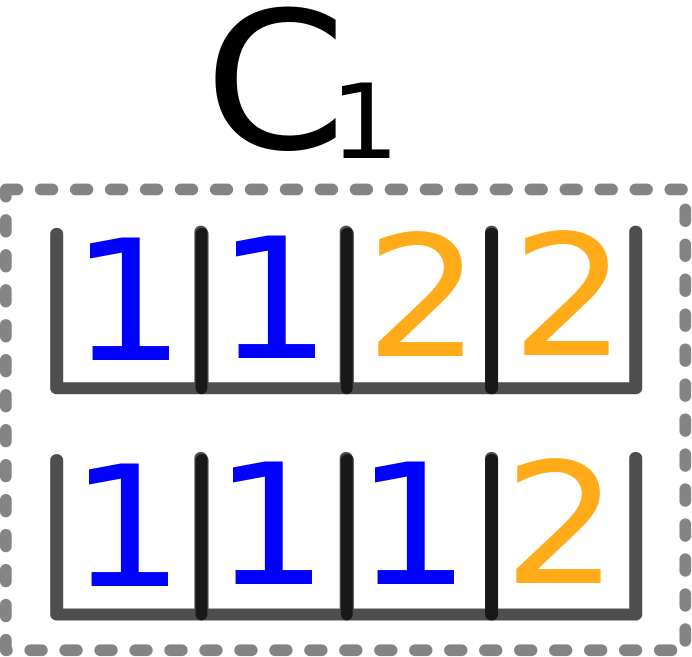
\includegraphics[width=2cm]{graficos/c1.png}
  \end{center}
\end{wrapfigure}

 El conjunto $C_{1}$ no es una solución válida ya que no cumple con la tercera condición. Para $i$=0, $j$=1, no existe una lista $l$ donde $l[i] \neq l[j]$.
\\
\\
\\

\begin{wrapfigure}{l}{3cm}
  \vspace{-41pt}
  \begin{center}
    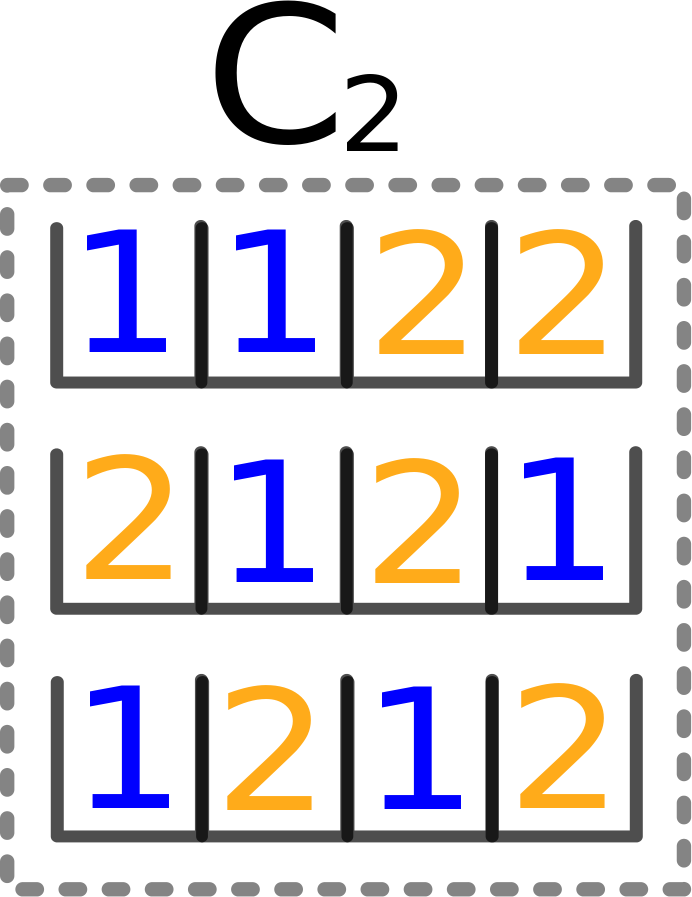
\includegraphics[width=2cm]{graficos/c2.png}
  \end{center}
\end{wrapfigure}

 El conjunto $C_{2}$ tampoco es una respuesta correcta ya que omitiendo alguna de las listas el conjunto sigue cumpliendo con las tres condiciones nombradas anteriormente. \\
 \\
 \\

{\begin{tabular}{ccc}
   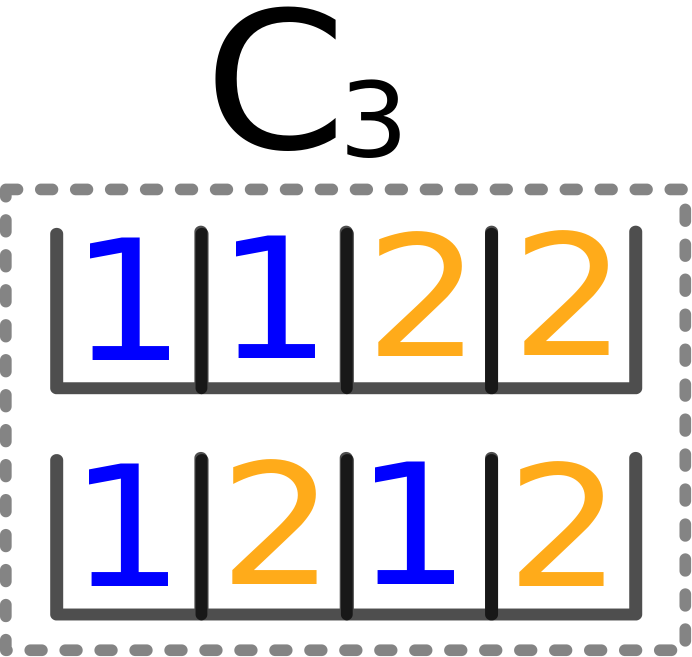
\includegraphics[height=2cm]{graficos/c3.png} & 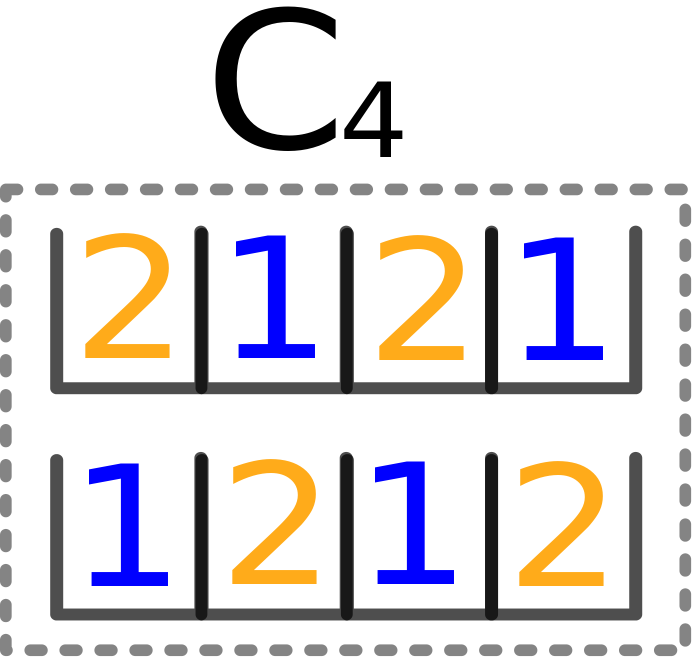
\includegraphics[height=2cm]{graficos/c4.png} & 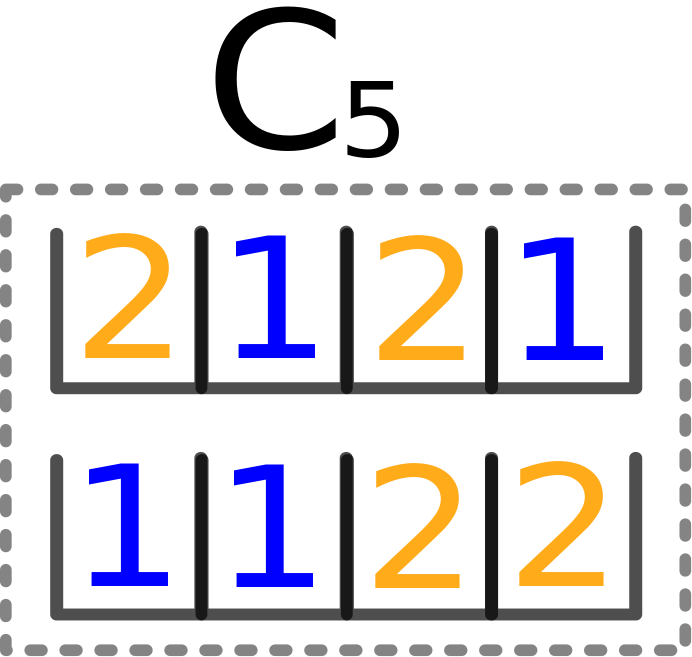
\includegraphics[height=2cm]{graficos/c5.png} \\
   \\

\end{tabular}}

  Los conjuntos $C_{3}$, $C_{4}$ y $C_{5}$ son respuestas válidas. 




    \subsection{Desarrollo}

        Para empezar, vamos a probar que para todo $n$, la menor cantidad de peleas necesarias es $\lceil log_{2}(n) \rceil$ por inducción en $N$.

        Caso Base: N = 1
        Un solo guerrero necesita $0$ peleas para haber peleado con todos los demás, $\lceil log_{2}(1) \rceil$ = $0$.

        Paso Inductivo: Supongo que $\forall$ $K$ $<$ $N$. La menor cantidad de peleas necesarias es $\lceil log_{2}(k) \rceil$. Quiero ver que se cumple también para $N$.

        Caso $N$ par:
        Genero una pelea $P$ de una mitad contra la otra. 

        {\begin{tabular}{ccc}
         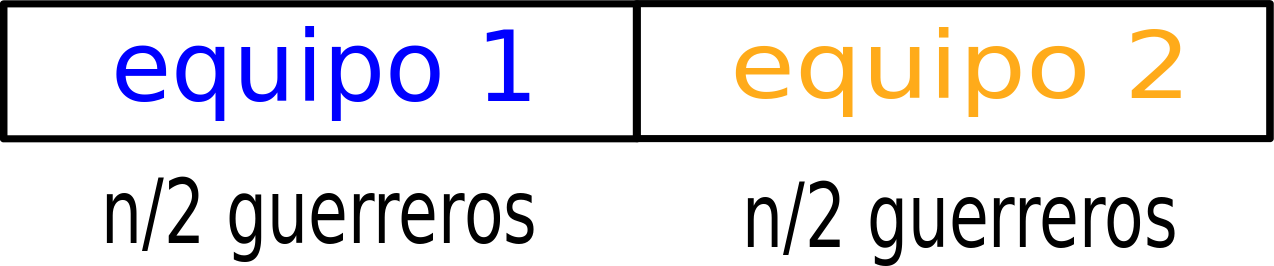
\includegraphics[height=1.5cm]{graficos/kaioken1.png} 

          \end{tabular}}

        Por Hipótesis Inductiva, cada subgrupo necesitaría $\lceil log_{2}(N/2) \rceil$ peleas para pelearse todos entre sí. Como estas subpeleas pueden hacerse “simultáneamente”, el total de peleas es $\lceil log_{2}(N/2) \rceil$ $+$ $1$. Esto es igual a $\lceil log_{2}(N) \rceil$. \\

        ¿Qué pasa si no divido a la mitad?\\


         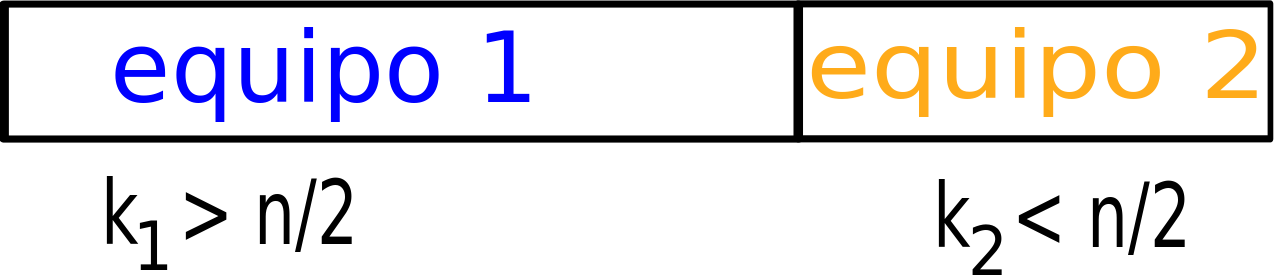
\includegraphics[height=1.5cm]{graficos/kaioken2.png} 
        
        

        En este caso, la cantidad de subpeleas previas depende de $k_{1}$, el de cantidad mayor entre las dos partes. Las peleas anteriores terminan siendo $\lceil log_{2}(k_{1}) \rceil$. Por hipótesis inductiva. Esto es mayor a $\lceil log_{2}(N/2) \rceil$. \\

        Caso N Impar: \\
        \\

         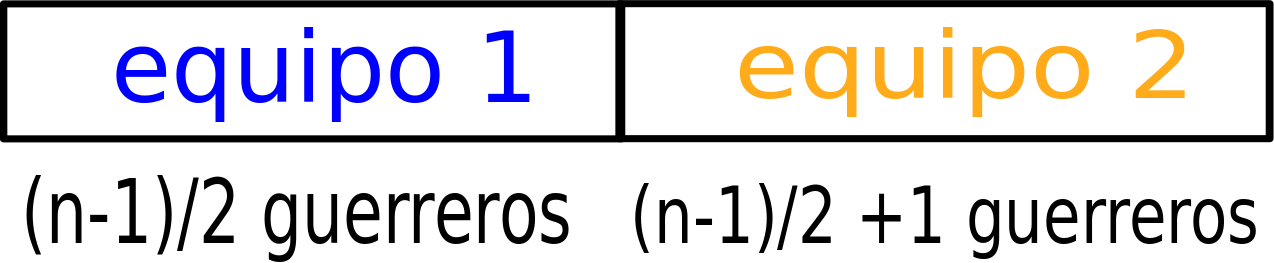
\includegraphics[height=1.5cm]{graficos/kaioken3.png} 
        
        

        Por hipótesis inductiva, podemos hacer pelear cada equipo entre sí en como mínimo $\lceil log_{2}((N-1)/2+1) \rceil$ $=$ $\lceil log_{2}((N+1)/2) \rceil$. Como $N$ es impar, $\lceil log_{2}((N+1)/2) \rceil$ es igual a $\lceil log_{2}(N/2) \rceil$. De esa manera, nos vuelve a quedar como cantidad de peleas total $\lceil log_{2}(N) \rceil$. \\

        Un corte de tamaños distinto a éste genera el mismo resultado que el caso par explicado anteriormente. \;






    \subsection{Complejidad}

    \begin{algoritmo}{kaioken}{int n}{int}

  \tipo{int} $cantMinPeleas \gets \lceil log_{2}(n) \rceil$ \com*{O(1)}
  \tipo{int} $equipo$ \com*{O(1)}

  \For(\com*{O($log_{2}(n)$)}){($i$ = 1; $i \leq cantMinPeleas$; $i$++)}{
    $equipo \gets 1$ \com*{O(1)}
    \For(\com*{O($n/2^{i-1}$)}){($h$ = 1; $h \leq n$; $h$ = $h + 2^{i-1}$)}{
      \For(\com*{O($2^{i-1}$)}){($k$ = 0; ($k < 2^{i-1}$) $\&$ ($h+k \leq n$); $k$++)}{
        escribir($equipo$) \com*{O(1)}
      }
        \eIf(\com*[f]{O(1)}){$equipo == 1$}{
          $equipo \gets 2$ \;
        }{
          $equipo \gets 1$ \;
        }
    }
  }


\end{algoritmo}

El segundo ciclo junto con el tercer ciclo tienen complejidad O($n$), ya que se multiplica O($n/2^{i-1}$) por O($2^{i-1}$). Entre los dos ciclos se recorren todos los guerreros una vez. El segundo recorre por grupos de guerreros que van a pertenecer al mismo equipo y el segundo de ellos le asigna a cada guerrero de un grupo el número de equipo correspondiente. 

Por ejemplo, para $n$=8, el ciclo número dos recorre como indican las flechas rojas para la pelea 1, 2 y 3 respectivamente. El tercer ciclo, avanza por los enemigos entre las flechas rojas. Se puede observar que el vector se recorre una sola vez para cada pelea. 


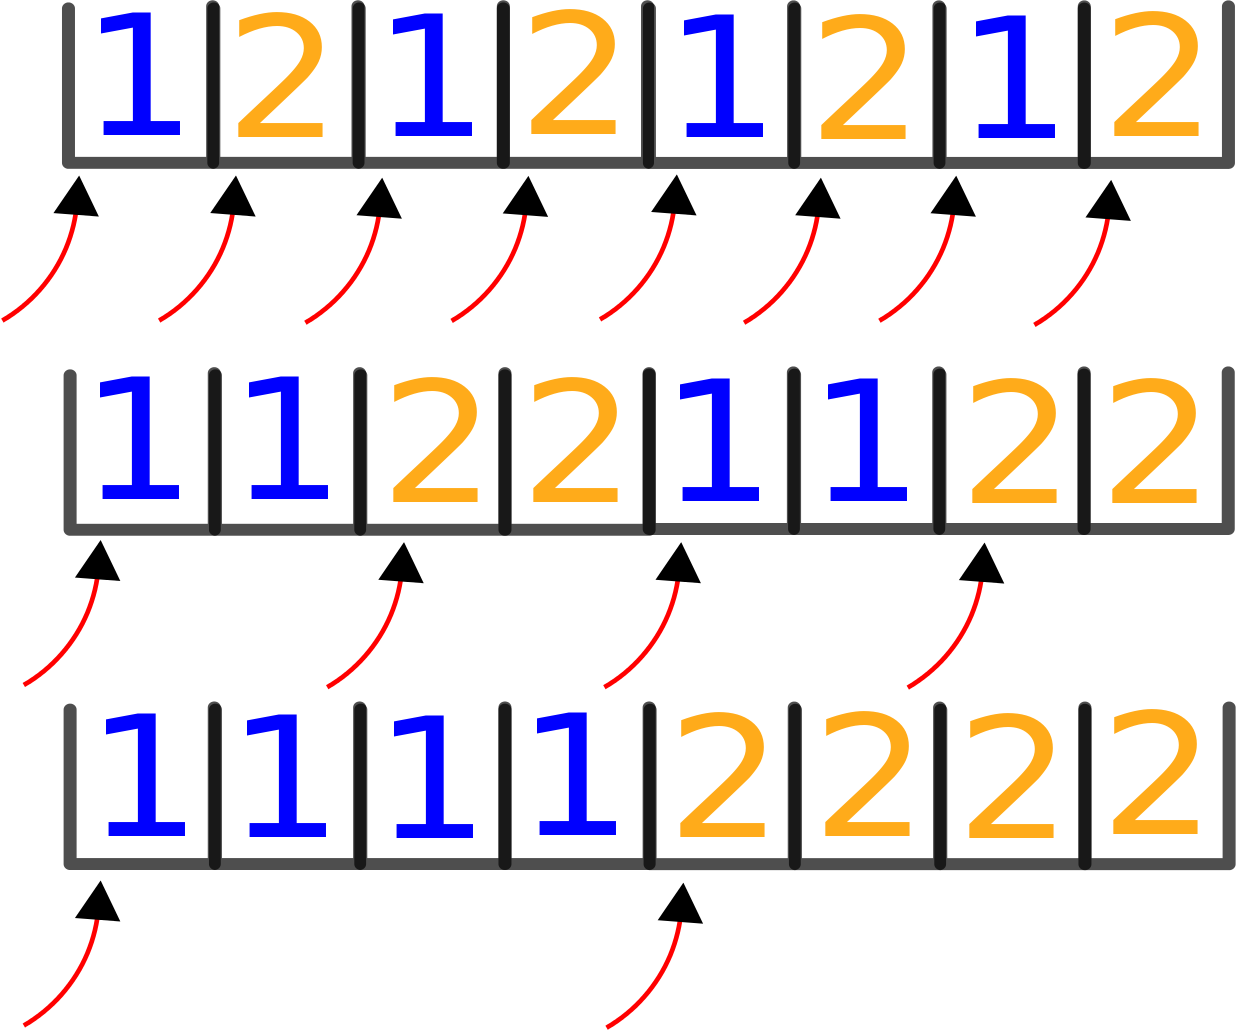
\includegraphics[height=4cm]{graficos/ciclo.png}


    \subsection{Código}


    \subsection{Experimentación}
		El objetivo de este experimento fue extraer conclusiones acerca de la variación en el tiempo de cómputo requerido por el algoritmo para distintos valores de $n$, con el fin de determinar su complejidad. 
    Para lograrlo, se graficó la curva $n \times log_{2}n / 13000000$ y se la comparó con las mediciones obtenidas al ejecutar el programa.

    \subsubsection*{Datos de entrada}
    La cantidad guerreros tomados fueron  desde 10000 hasta 300000 de 10000 en 10000.
    El archivo necesario para ejecutar el experimento se encuentra en la carpeta exp/kaioken con nombre kaioken.sh. 
		Para realizar las mediciones se  utilizaron las funciones provistas a tal efecto por la cátedra. Además, para evitar posibles errores en las mismas, cada una se repitió 7 veces, considerando luego el promedio entre los valores obtenidos. 



      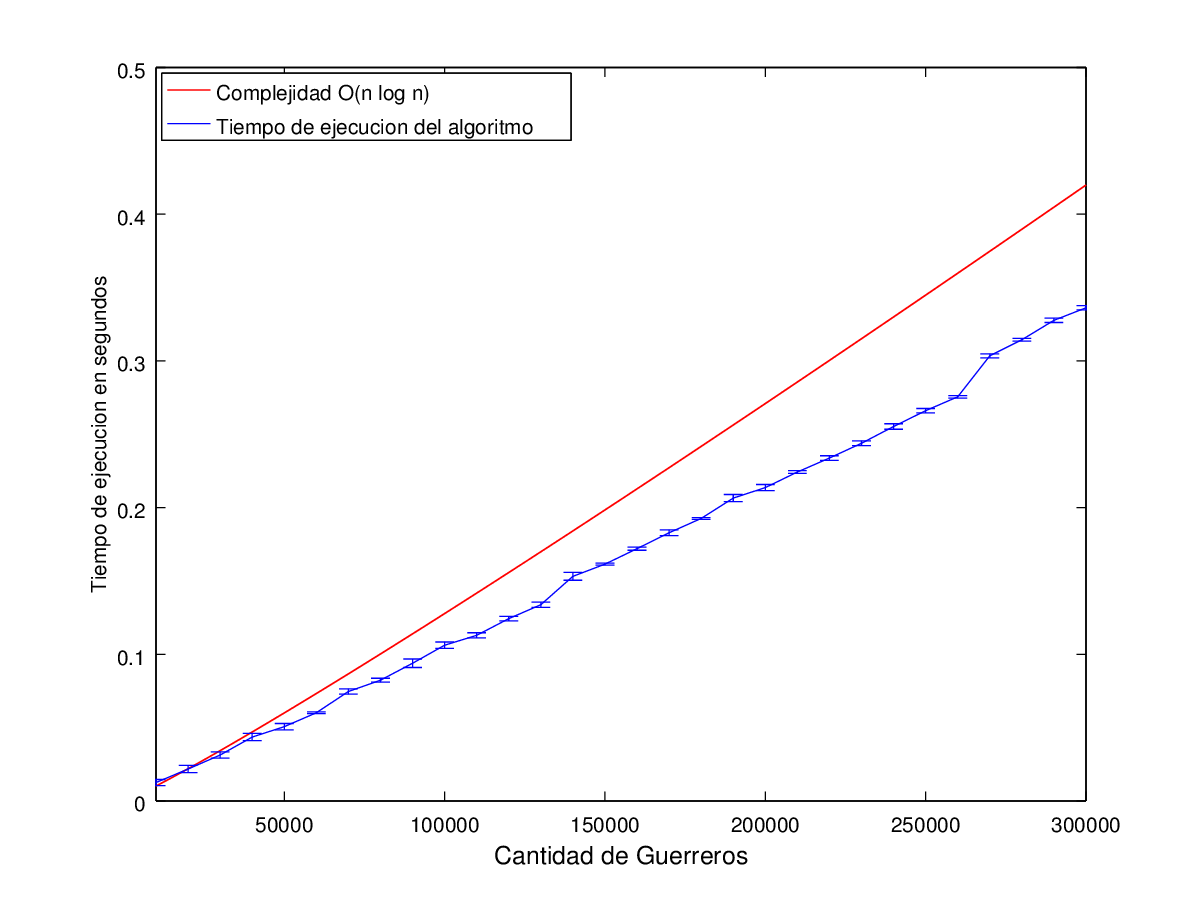
\includegraphics[height=11cm]{graficos/kaioken-exp.png}



		\subsubsection*{Conclusión}
			Se puede observar en el gráfico que la curva $n \times log_{2}n / 13000000$ está por encima de la curva que forman las mediciones del tiempo de ejecución del programa. Por lo tanto, se demuestra empiricamente que la complejidad del programa es O($n \times log_{2}n$)

\clearpage
\section{Genkidama}

	\subsection{Introducción}

	
    \subsection{Desarrollo}
    	
    	Para demostrar que este algoritmo resuelve el problema de manera eficiente utilizaremos dos lemas:
    		\subsubsection*{Lema 1}

    			Sean $v_{i}$, $v_{j}$ las coordenadas de dos guerreros enemigos. Si se lanza una Genkidama a $v_{j}$ y con la explosión de la misma también muere $v_{i}$, entonces $ \forall h \in (i,j), v_{h}$ morirá también. 

    		\subsubsection*{Demostración Lema 1}

    			Sean $v_{i}$ = ($x_{i}$, $y_{i}$), $v_{j}$ = ($x_{j}$, $y_{j}$) y $v_{h}$ = ($x_{h}$, $y_{h}$) posiciones de guerreros enemigos con $i < j < h$.
    			Sabemos que $x_{i} > x_{j}$ y $y_{i} < y_{j}$ porque las $x$ son decrecientes y las $y$ crecientes.

    			Quiero ver que $x_{j} + T \geqslant x_{h}$ y que $y_{j} + T > y_{h}$.

    			Veamos primero que $x_{j} + T \geqslant x_{h}$:

    			Sabemos que $x_{j} + T \geqslant x_{i}$ porque disparando en $x_{j}$ muere $x_{i}$ y además $x_{i} > x_{h}$ entonces juntando éstas dos propiedades podemos asegurar que $x_{j} + T > x_{h}$.

    			Ahora veamos que $y_{j} + T > y_{h}$:

    			Sabemos que $y_{j} > y_{h}$ y como $T > 0$ entonces $y_{j} + T > y_{h}$.

    			Entonces queda demostrado que todos los gurreros que se encuentren entre $v_{i}$ y $v_{j}$ mueren cuando se lanza una Genkidama a $v_{j}$.

    		\subsubsection*{Lema 2}

    			Sean $j$ y $k$ posiciones de guerreros enemigos tal que disparandole al que se encuentra en la posición $j$ el elemento de mayor índice que muere es el de la posición $k$, si le disparo a $i$ (con $i < j$) no puede morir el de la posición $k+1$.


    		\subsubsection*{Demostración Lema 2}
    			Demostración por el absurdo:

    			Como disparandole al soldado de la posición $j$ mata al de la posición $k$ entonces sabemos que $x_{j} - T \leq x_{k}$.
    			Como disparandole al guerrero de la posición $j$ no mata al de la posición $k+1$ entonces $x_{j} - T > x_{k+1}$
    			También sabemos que $x_{j} < x_{i}$ porque las $x$ son decrecientes.

    			Supongamos que disparando en la posición $i$ mato al enemigo de la posición $k+1$, entonces $x_{i} - T < x_{k+1}$.
    			entonces tenemos que $x_{j} - T > x_{k+1}$ y además $x_{i} > x_{j}$. Por esto último, si restamos $T$ en ambos lados queda que $x_{i} - T > x_{j} - T$, pero sabiamos que $x_{j} - T > x_{k+1}$ entonces $x_{i} - T > x_{k+1}$ lo que es absurdo porque contradice la hipótesis. 
    			Por lo tanto $x_{i}$ no puede matar a $x_{k+1}$. \\
    			\\
    			\\


		Es fácil ver que con esta forma de resolución se mueren todos los enemigos ya que se toma el primer guerrero y se busca cual es la posición mas lejana a la cual puedo lanzar una genkidama y aun así matar al guerrero en cuestión. Por el lema 1, todos los guerreros que se encontraban entre el primero y el soldado a quien se le disparó también morirán. Luego se avanza hasta el primer enemigo que haya quedado vivo del lado derecho y se repite el mismo procedimiento partiendo del primer enemigo que sobrevivió al ataque. \\ 


		Veamos ahora que esta es la forma óptima de arrojar las Genkidamas:\\


		Como seguro en algún momento va a ser necesario matar al primero entonces vamos a matarlo tirando la Genkidama en un lugar estratégico generando que mueran la mayor cantidad de guerreros posibles junto con el enemigo en cuestión. Para ello, la manera mas eficiente de disparar la genkidama es buscar cual es el último guerrero a quien se le pueda disparar desde el cual siga matando al primero, ya que cualquier otro disparo genarará una menor o igual cantidad de muertes.\\
		Sean $i$, $j$, $k$ guerreros enemigos donde $j$ representa el último guerrero al que le puedo disparar para matar a $i$. $k$ es el último guerrero que muere cuendo lanzo la Genkidama en $j$.\\
		Por el lema 2 se sabe que si disparo en cualquier guerrero que se encuentre entre $i$ y $j$ puede pasar que mate a $k$ o no, pero nunca puede pasar que mate al soldado que se encuentra en la posición $k+1$. Entonces si disparo la Genkidama en un $x_{h}$ con $h \in (i, j)$ no mato mas guerreros de los que mataba tirándola en $x_{j}$ del lado derecho, pero si puede pasar que mate menos, por ejemplo cuando no mata al $x_{k}$.\\
		Por lo tanto ésta es una de las formas óptimas de tirar la Genkidama para matar al primer soldado enemigo.\\
		Como el algoritmo se repite cada vez que es lanzada una Genkidama tomando como guerrero nicial el último que quedo vivo, entonces debemos volver a dispararle a este de la forma mas eficiente posible. Por lo tanto el algoritmo es eficiente.  \\

		\subsubsection*{Descripción}
		 
	   	Como el objetivo es matar a todos realizando la menor cantidad de disparos, lo que vamos a hacer es buscar cual es el último guerrero a quien se le pueda disparar desde el cual siga matando al primero de la lista. Allí será donde se disparará la primer Genkidama. Una vez realizado el disparo se buscará cual es el primer soldado que sobrevivió al ataque y se reiniciará el problema tomando a ese guerrero como el nuevo primero. Éste proceso se repetirá hasta que no queden mas guerreros enemigos vivos. \\

		
		MataAl:
		Ésta función recibe por parámetro el valor del $T$,  un vector de puntos en el plano que representa los guerreros enemigos y dos enteros que representan posiciones en el vector.  El resultado es un booleano que indica si disparándole una Genkidama al enemigo ubicado en la posición $i$ mata al de la posición $j$ también.\\

		\begin{algoritmo}{MataAl}{\In{i}{int}, \In{j}{int}, \In{N}{int}, \In{T}{int}, \Inout{enemigos}{vector(pair(int,int))} }{bool}
		  \eIf{cuando disparo al que esta en la posición $i$ mata al que esta en la posición $j$}{
    		devolver true \;
  				}{
    		devolver false \;
  			}

		\end{algoritmo}
		
		MasLejanoQueMata:
		Ésta función recibe por parámetro el valor del $T$, un vector de puntos en el plano que representa los guerreros enemigos y un entero que indica la posición de un soldado en el vector.
		La función devuelve la posición del ultimo guerrero que muere en caso de dispararle al que ocupa la posición pasada por parámetro.\\

		\begin{algoritmo}{masLejanoQueMata}{\In{aEsteLeDisparo}{int}, \In{N}{int}, \Inout{enemigos}{vector(pair(int,int))}}{int}
			j = i + 1;\;
			\While{si le disparo al que esta en la posición $i$ mata al que está en la posición $j$}{
    		j++ \;
  			}
  			devolver j - 1; // Cuando sale del ciclo $j$ el la posición del primer guerrero que queda vivo en caso de dispararle al que ocupa la posición $i$ entonces hay que restarle uno para devolver la posición del último que muere.\;
		\end{algoritmo}

		
		MasLejanoQueMataAl:
		Ésta función recibe por parámetro el valor del $T$,  un vector de puntos en el plano que representa los guerreros enemigos y un entero que indica la posición de un soldado en el vector.
		La función devuelve la posición del ultimo guerrero al cual puedo disarale pero que siga matando al enemigo que ocupa la posicion pasada por parametro.\\ 

	\begin{algoritmo}{masLejanoQueMataAl}{\In{i}{int}, \In{N}{int}, \In{T}{int}, \Inout{enemigos}{vector(pair(int,int))}}{int}
		j = i + 1 \;
		\While{si le disparo al que esta en la posición $j$ sigue matando al que esta en la posición $i$}{
    		j++ \;
  		}
  		j = j - 1;\; //cuando sale del ciclo $j$ es la posición del primer guerrero al que hay que dispararle y que no mate al $i$. Como tiene que matarlo se retrocede uno. 

	\end{algoritmo} \;

		
		Genkidama:
		Ésta función recibe por parámetro el valor del $T$,  un vector de puntos en el plano que representa los guerreros enemigos y su longitud, y un puntero a una lista de enteros donde se guardarán los guerreros a los cuales será necesario lanzar genkidamas. Devolverá tambien la cantidad de disparos realizados. \\

	\begin{algoritmo}{genkidama}{\In{N}{int}, \In{T}{int}, \In{enemigos}{vector(pair(int,int))}, \Inout{DisparosEfectuados}{list(int)}}{int}

		int cantGenkidamas=0;
  		int i=0;
  		\While{$i < n$}{
    		int aEsteLeDisparo=masLejanoQueMataAl(i,N,T,enemigos);//busco el mas lejano que mate al primero de los que quedan vivos \;
    		i = masLejanoQueMata(aEsteLeDisparo,N,T,enemigos) + 1;//empiezo a preguntar desde el sigiente al ultimo en morir\;
    		agregar AEsteLeDisparo a la lista de disparos efectuados;\;
    		cantGenkidamas++; \;
  		}
  		devolver cantGenkidamas; \;
	\end{algoritmo} \;
	



    \subsection{Complejidad}


    \subsection{Código}


    \subsection{Experimentación}


    	\subsubsection*{Experimento 1}\;
			En este experimento se analizará la variación del tiempo de ejecución del algoritmo cuando varía la cantidad de guerreros enemigos dejando fijo el parámetro $T$. Para ello se generarán diferentes archivos con las coordenadas de los enemigos, uno por cada tamaño de bando contrario. Las coordenadas de los soldados serán aleatorias tomando una cota como máximo valor posible para las variables x e y. Luego pasando esos archivos como parámetro de entrada al problema de genkidama, se medirán los tiempos de ejecución. \;

		\subsubsection*{Datos de entrada}\;
			Los tamaños del bando enemigo tomados fueron  desde $50$ hasta $1000$ de $50$ en $50$. \;
			El valor de $T$ utilizado fue $50$.\;
			Para generarlos se utilizó el generador.cpp que se encuentra en la carpeta exp/genkidama/exp1 y para correrlo se utilizó el exp1.sh que se encuentra en la misma carpeta. \;
			Con el fin de acercarse a los valores reales y descartar posibles falsos resultados, se ejecuta la resolución del problema para cada uno de los tamaños de equipo siete veces y se calcula el promedio de los tiempos medidos.\;

      	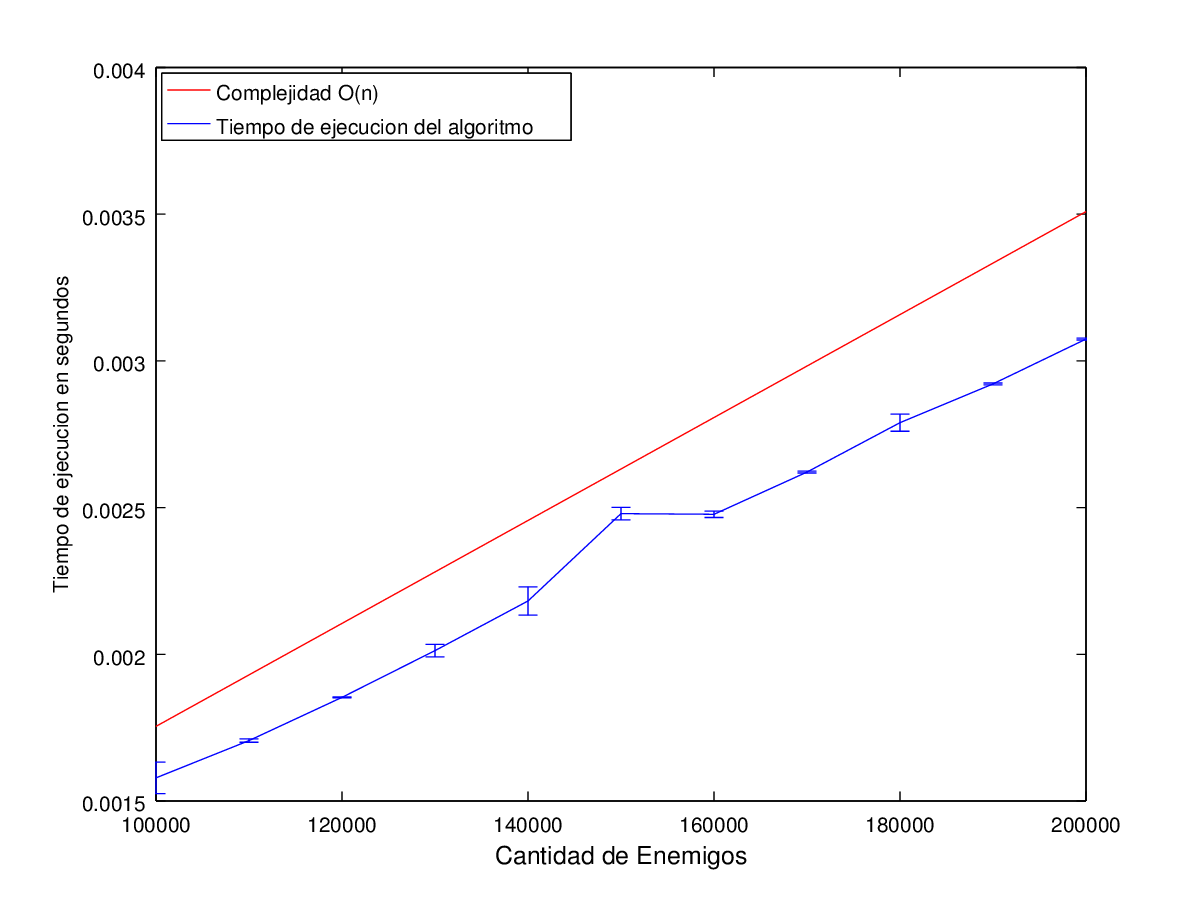
\includegraphics[height=11cm]{graficos/genkidama-exp1.png}


    	\subsubsection*{Conclusiones}
			Como se puede observar en el gráfico, el tiempo de ejecución aumenta de manera lineal con respecto a la cantidad de guerreros enemigos. Esto es así ya que el algoritmo recorre todos los puntos sin importar la distancia que haya entre ellos y la cantidad de disparos a realizar. Por ello podemos asegurar que la complejidad es de o(N).
			\\



		\subsubsection*{Experimento 2}\;
			En este experimento vamos a observar como varia el tiempo de ejecución para diferentes valores del parámetro $T$ dejando constante la cantidad de guerreros enemigos.\;


		\subsubsection*{Datos de entrada}

		
			Los valores de $T$ utilizados fueron $50$ $70$ $80$ $90$ $100$ $120$ $130$ $140$ $150$ $170$ $190$ $200$.\;
			La cantidad de guerreros en el equipo contrario utilizada fue 1000
			Para generarlos se utilizó el generador.cpp que se encuentra en la carpeta exp/genkidama/exp2 y para correrlo se utilizó el exp2.sh que se encuentra en la misma carpeta.\;
			Con el fin de acercarse a los valores reales y descartar posibles falsos resultados, se ejecuta la resolución del problema para cada uno de los valores de $T$ siete veces y se calcula el promedio de los tiempos medidos.\;
      	

      	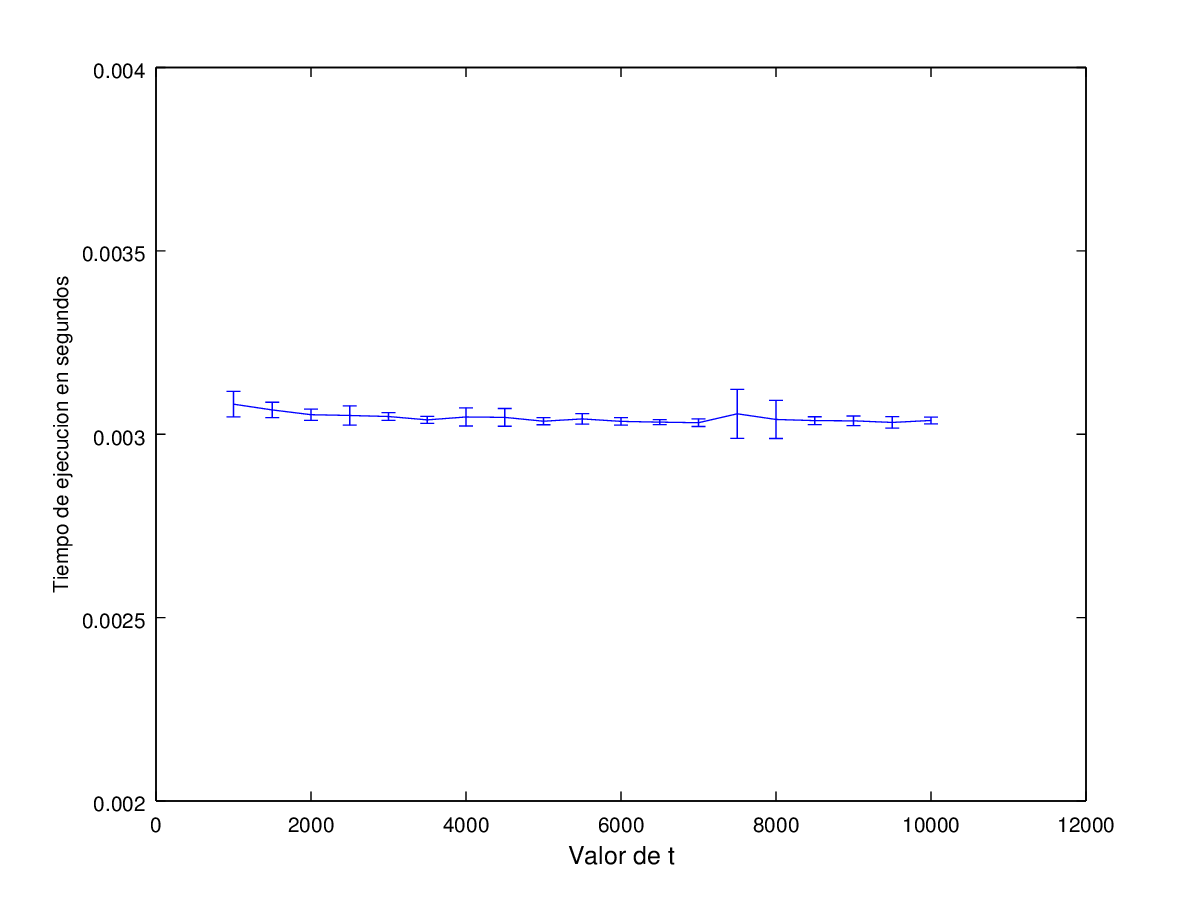
\includegraphics[height=11cm]{graficos/genkidama-exp2.png}

    	
    	\subsubsection*{Conclusiones}


			Como se puede observar,las variaciones en el tiempo de ejeucion para cada $T$ son despreciables por lo tanto se puede decir que no importa como varia el $T$, el tiempo que tarda en ejecutar el algoritmo es el mismo cuando la cantidad de puntos no varia.\;

		\;

    	\subsubsection*{Experimento 3}

			En este experimento vamos a observar como varia el tiempo de ejecución del algoritmo para casos bordes. En el primero tomaremos guerreros que se encuentren a muy poca distancia  unos de otros y en el segundo los enemigos estarán separados por grandes distancias, dejando siempre constante la cantidad de soldados. Luego mediremos los tiempos de ejecución del algoritmo genkidama para ambos casos tomando un valor de $T$ grande y luego uno chico.\;

		
		\subsubsection*{Datos de entrada}


			Los valores de $T$ utilizados fueron $4$ y $50$.
			La cantidad de guerreros en el equipo contrario utilizada fue 1000.
			En el primero las distancias eran de 2 entre soldados y en el segundo de $50$.
			Para generarlos se utilizó el generadorJuntos.cpp y el generadorSeparados.cpp  que se encuentran en la carpeta exp/genkidama/exp3.
			Para correrlo se utilizó el exp3.sh 
			Con el fin de acercarse a los valores reales y descartar posibles falsos resultados, se ejecuta la resolución del problema para cada uno de los valores de $T$ siete veces y se calcula el promedio de los tiempos medidos.\;


      	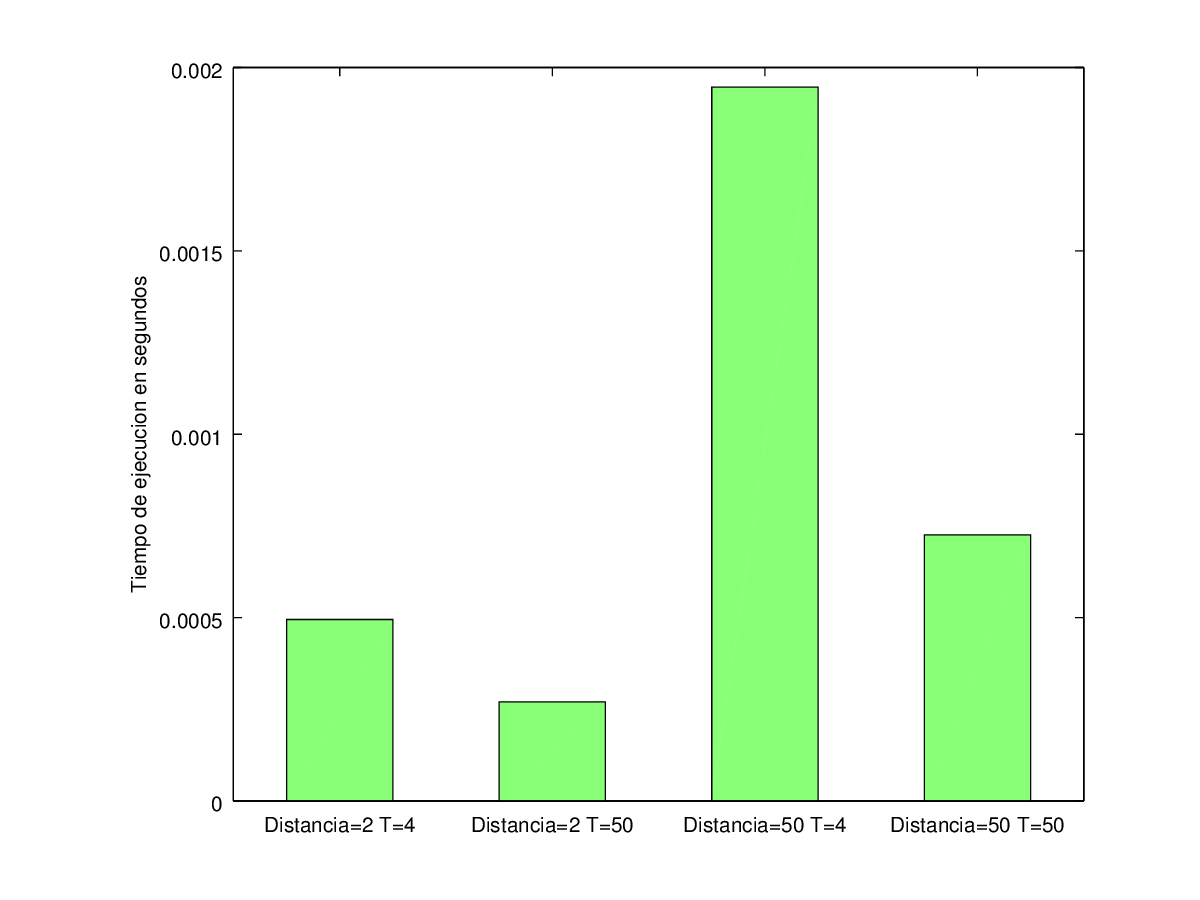
\includegraphics[height=11cm]{graficos/genkidama-exp3.png}


    	\subsubsection*{Conclusiones}\;

			Como se puede observar en el gráfico, cuando los puntos se encuentran muy distantes unos de otros y se utiliza un valor de $T$ muy chico el tiempo de ejecución es muy alto. 
			Esto se debe a que el algoritmo toma el primer guerrero y se fija cual es el ultimo al cual puede disparar si quiere matar al primero recorriendo todos los que confirmen este hecho y luego retrocediendo uno cuando le dicen que no. Luego dispara la genkidama, y avanza hasta el primer guerrero que haya sobrevivido y vuelve a comenzar. Esto se repite hasta que no queden guerreros vivos. En el caso de que todos los guerreros se encuentren a tanta distancia como para que sea necesario lanzar una genkidama por cada uno de ellos entonces el algoritmo avanzará de a uno y en cada paso avanza y retrocede uno generando así que la complejidad sea de $\mathcal{O}(2N)$. 

\clearpage
\section{Kamehameha}

	\subsection{Introducción}
		El problema a resolver nos pide encontrar una posible forma de cubrir N puntos en un plano con la menor cantidad de rectas posible.
		Es decir: Minimizar la cantidad de rectas necesarias para cubrir N puntos dados.
		Notamos que encontrar un conjunto de rectas optimo que contenga al conjunto $\mathcal{P}tos$ (El conjunto de puntos dado),de que una recta queda definida univocamente dando 2(dos) puntos pertenecenecientes. El problema entonces que resolveremos sera encontrar un conjuntos de pares $\mathcal{CP}ares	    \subseteq \mathcal{P}tos \times \mathcal{P}tos$ de modo tal que las rectas inducidas por $\mathcal{CP}ares$ contengan a todo $p \in \mathcal{P}tos$ y ademas $\nexists \quad \overline{\rm \mathcal{CP}ares} / \quad \textrm{queden  inducidas rectas que contenga a todo} \quad \mathcal{P}tos$ con  $\# \overline{\rm \mathcal{CP}ares} < \# \mathcal{CP}ares$. \\
		Es este entonces el problema principal que resolveremos.\\
		Margen de notación: la recta que induce $(p,p) \in \mathcal{P}tos \times \mathcal{P}tos$ es alguna que pasa por p pero que no influye en lo otros puntos.
	
    \subsection{Desarrollo}
    	Para resolver este problema implementaremos un algoritmo de Backtracking. En el cual, el papel principal lo juega la funcion ``mejoresPares'' que es la encargada de devolver un conjunto optimo de pares que inducen las rectas que cubren todos los puntos de alguna de las maneras optimas posibles.
  		procederemos entonces a mostrar un pseudocodigo de esta funcion, (por claridad utilizaremos las funciones tradicionales de conjuntos para operar pero en realidad todos los conjuntos estan implementados sobre vectores lo que les da un caracter numerable y por lo tanto la operacion [ ]) :
  		\\ \\
  		$mejoresPares(conjunto \quad Puntos) \longmapsto conjuntoParesOptimo $\\
  		$mejoresPares(\emptyset) \equiv \emptyset$\\
  		$mejoresPares(\{ p \}) \equiv \{ (p,p) \} $\\
     	$mejoresPares(\{ p,q \}) \equiv \{ (p,q) \} $\\
     	$mejoresPares(\{ p \} \cup Ptos) :$\\
     	$Pares \gets generarConjPares(p,Ptos)$ //genero los posibles pares que pasan por p \\ \\
     	$i \gets \{0..\#Pares\}$  // genero por cada $par_i$ los mejores pares desde los LI con $par_i$
		\\
 		$\quad posiblesConvinaciones[i]=mejoresPares(sinLD(Pares[i],Ptos))$\\ 
 		\\
 		$return \gets conjMasChico(posiblesConvinaciones)$ // devuelve el conjunto de pares mas chico que tenga
		\\
		\\
		Se ve en el pseudocodigo que esencialmente lo que hacemos es generar todas las posibles rectas que pasan por punto y luego tomar la que cuando sacas los puntos que le pertenecen te quda el conjunto cuya cantidad de rectas optimas para cubrirlo sea menor. En otras palabras tomo la recta a la cual al aplicarle el algoritmo recursivamente termine teniendo la menor cantidad de pares en el conjunto que induce sus rectas.\\
		De tener el conjunto de rectas optimo solo tengo que adaptarlo con algunas operaciones $\mathcal{O}(n)$ muy sencillas para obtener la salida requerida en el ejercicio, ya que es simplemente ver quienes estan en cada recta, contarlos y asegurarme de no repetirlos si otra recta pasa por algun punto que ya tome en cuenta.
		\\ 
		\\
		En cuanto a la correctitud de la solucion, es evidente que este algoritmo funciona, osea que la convinacion de rectas es optima pues para econtrarla se la comparo con todas las posibles convinaciones de rectas que cubren a todos los posibles pares de puntos y se elegio de entre ellos el conjunto de rectas con el menor cardinal.


    \subsection{Complejidad}

    	La complejidad requerida de $\mathcal{O}(N^{N+2})$ se cumple pues, si analizamos es codigo se ve que en cada llamada recursiva se realizan operaciones de a lo sumo $\mathcal{O}(N^{2})$ ya que generar conjunto de pares que pasen por un punto es $\mathcal{O}(N)$ (el punto en cuestion juntarlo con los n-1 restantes), generar un conjunto sin Linearmente dependientes con un punto tambien es $\mathcal{O}(N)$ (pues es chequear una igualdad en  $\mathcal{O}(1)$ para cada punto) y esto se ejecuta a lo sumo N veces lo que no supera entonces la complejidad $\mathcal{O}(N^{2})$ y realizar buscar un minimo sobre un vector de n elementos es tambien $\mathcal{O}(N)$. \\
		Por otro lado si vemos la cantidad de llamadas recursivas que se realizan, el esquema seria:\\
		En la primer iteracion se generan N llamadas recursivas una para cada par considerado.\\
		-En el segundo nivel de llamada cada una de las N llamadas genera n-2 llamadas (pues trabajan sobre un conjunto de puntos al que le falta un par). \\ 
		Continua asi entonces en cada nivel llamando a menos llamadas hasta llegar a los casos base.
		Si bien basado en el esquema planteado se observa que podriamos acotar la complejidad del algorimo por un tiempo factorial si hilaramos fino. De manera mas sencilla aun se ve que se puede acotar la cantidad de llamadas recursivas por $N^{N}$ dando una complejidad de la funcion ``mejoresPares'' de a lo sumo $\mathcal{O}(N^{N+2})$ pues es la multiplicacion de la cantidad de llamadas por el lo que tarda cada una.Y como el resto del codigo no utiliza funcion con niguna complejidad relevante (no pasa el $\mathcal{O}(N^{2})$ la parte no recursiva) entonces podemos concluir que el algoritmo $ \in \mathcal{O}(N^{N+2})$.


    \subsection{Código}


    \subsection{Experimentación}

    	\subsubsection*{Experimento 1}\;

    		En este experimento se analizará la variación del tiempo de ejecución del algoritmo cuando varía la cantidad de guerreros enemigos. Para ello se generarán diferentes archivos con las coordenadas de los enemigos, uno por cada tamaño de bando contrario. Las coordenadas de los soldados serán aleatorias tomando una cota como máximo valor posible para las variables x e y. Luego pasando esos archivos como parámetro de entrada al problema de kamehameha, se medirán los tiempos de ejecución. \;

    	\subsubsection*{Datos de entrada}\;
    		Los tamaños del bando enemigo tomados fueron $5$ $7$ $9$ $10$ $11$ $12$ $13$ $14$ $15$ $16$ $17$ $18$.
			Para generarlos se utilizó el generador.cpp que se encuentra en la carpeta exp/kamehameha/exp1 y para correrlo se utilizó el exp1.sh que se encuentra en la misma carpeta. \;
			Con el fin de acercarse a los valores reales y descartar posibles falsos resultados, se ejecuta la resolución del problema para cada uno de los tamaños de equipo siete veces y se calcula el promedio de los tiempos medidos.\;

      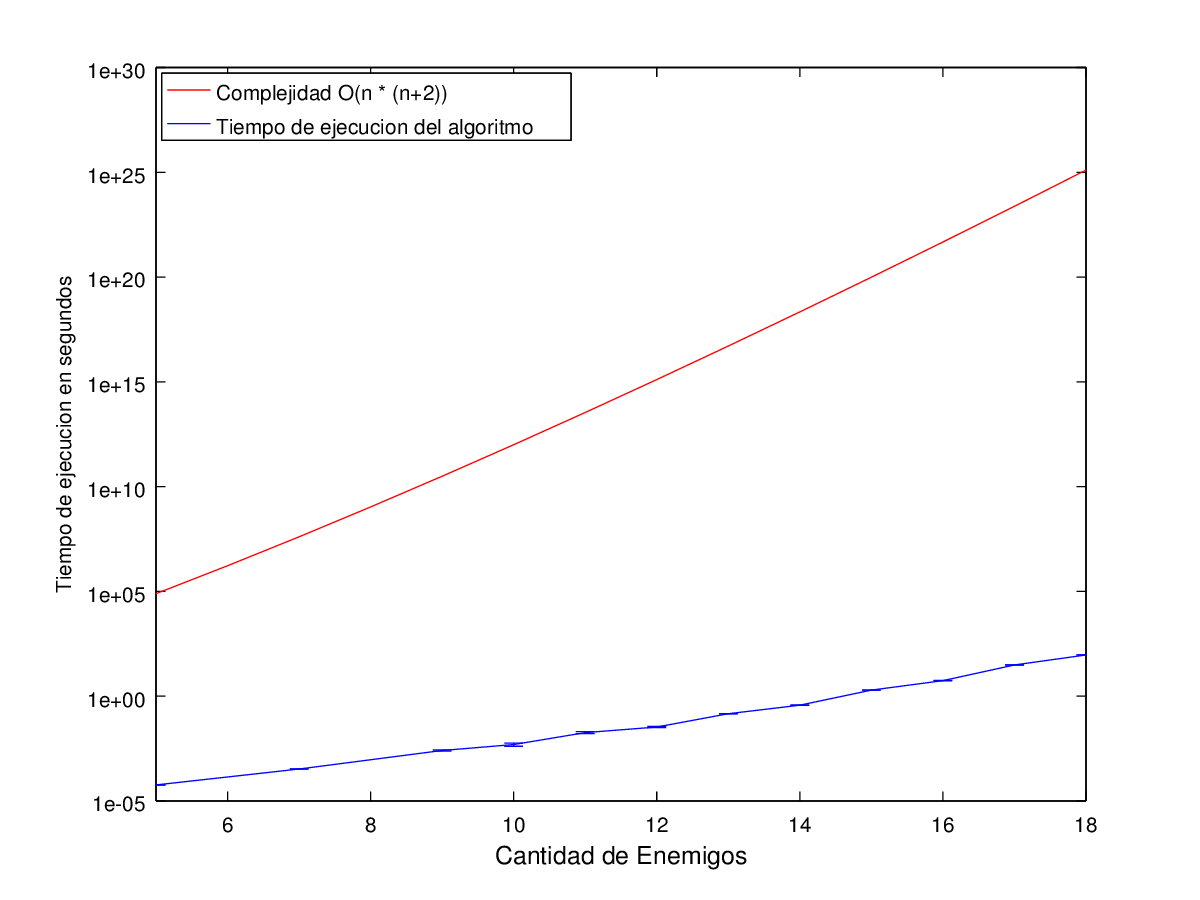
\includegraphics[height=11cm]{graficos/kamehameha-exp1.png}



		\subsubsection*{Conclusiones}\;

			Como se puede observar en el gráfico, el tiempo de ejecución aumenta de manera exponencial con respecto a la cantidad de guerreros enemigos dando una complejidad de $\mathcal{O}(N^{N+2})$. Esto es así ya que el algoritmo busca todas las posibles combinaciones de disparos a efectuar y de todas ellas elige la que requiera menor cantidad de lanzamientos. \;

		\;
		\;
		
    	\subsubsection*{Experimento 2}\;
    		En este experimento vamos a comparar como varia el tiempo de ejecución del algoritmo para casos bordes. En el primero tomaremos guerreros que se encuentren dispuestos de forma alineada de manera que con un solo disparo se pueda matar a todo el equipo enemigo. En el segundo, los guerreros estarán distribuidos de forma tal que solo se pueda matar de a dos de ellos con un disparo. Tomaremos la misma cantidad de soldados del bando enemigo para ambos casos. \;

    	\subsubsection*{Datos de entrada}\;
    		El tamaño del bando enemigo utilizado fue de 18 guerreros.
			Para generar el primer caso se utilizó el generador.cpp y para el segundo el generador2.cpp que se encuentran en la carpeta exp/kamehameha/exp2. Para correrlos se utilizó el exp2.sh que se encuentra en la misma carpeta.\;
			Con el fin de acercarse a los valores reales y descartar posibles falsos resultados, se ejecuta la resolución del problema para cada uno de los tamaños de equipo siete veces y se calcula el promedio de los tiempos medidos.\;

		\subsubsection*{Conclusiones}\;
			Como se puede ver en la tabla, el tiempo de ejecución cuando los puntos se encuentran alineados es mucho menos que cuando solo puedo matar de a dos guerreros enemigos. Esto se debe a que el algoritmo toma todos los posibles pares de guerreros y para cada uno de ellos se fija como armar mas pares sin tener en cuenta los soldados que quedan alineados con la recta que une al primer par. En el caso que estén todos alineados la complejidad bajará a $\mathcal{O}(N)$ ya que para ningún posible par que se pueda armar en un primer momento quedan mas guerreros que no se encuentren alineados con el primer par. Por lo que solo tomará posibles pares de guerreros y finalizará la ejecución. En cambio cuando están muy desalineados, por cada par inicial quedan exactamente $n - 2$ guerreros para reordenar en pares, generando así una complejidad de $\mathcal{O}(N^{N+2})$.



\clearpage

\section{Código}
\subsection{KaioKen}

\begin{lstlisting}
void kaioken (int cantGuerreros) {
  int cantMinPeleas = ceil(log2(cantGuerreros));
  int equipo;
  cout << cantMinPeleas << endl;
  for (int i = 1; i <= cantMinPeleas; i++) { 
    equipo = 1; 
    for (int h = 1; h <= cantGuerreros; h = h + pow(2, i-1)) {
        for (int k = 0; k <  pow(2,i-1) && (h + k <= cantGuerreros); k++ ) {
           cout << equipo << " ";
        }
        if (equipo == 1) {
            equipo = 2;
        } else {
            equipo = 1;
        }
    }
    cout << endl;
  }
}
\end{lstlisting}

\subsection{Genkidama}

\begin{lstlisting}
int genkidama (int N,int T,vector<pair<int,int> >& enemigos,
	list<int>* DisparosEfectuados){
  int cantGenkidamas=0;
  int i=0;

  while (i<N) {
    int aEsteLeDisparo=masLejanoQueMataAl(i,N,T,enemigos);
    i = masLejanoQueMata(aEsteLeDisparo,N,T,enemigos) + 1;
    DisparosEfectuados->push_back(aEsteLeDisparo);
    cantGenkidamas++;
  }
  return cantGenkidamas;
}

int masLejanoQueMataAl(int i,int N, int T,vector<pair<int,int> >& enemigos){
    int j=i+1;
    while(j<enemigos.size() && mataAl(j,i,N,T,enemigos)){
      j++;
    }
    return j-1;
}

int masLejanoQueMata(int aEsteLeDisparo, int N,int T,
 vector<pair<int,int> >& enemigos){
  int j=aEsteLeDisparo+1;
  while(j<enemigos.size() && mataAl(aEsteLeDisparo,j,N,T,enemigos)){
    j++;
  }
  return j-1;

}

bool mataAl(int i,int j,int N,int T,vector<pair<int,int> >& enemigos){
  if(enemigos[i].first + T >= enemigos[j].first && 
  	enemigos[i].second + T >= enemigos[j].second )
    return true;
  else
    return false;
}
\end{lstlisting}

\subsection{Kamehameha}

\begin{lstlisting}
int kamehameha(vector<pair<int,int> > puntos,
	vector<pair<pair<int,int>,pair<int,int> > >& paresOptimos){
   paresOptimos = mejoresPares(puntos);

    return paresOptimos.size();
}

vector<pair<pair<int,int>,pair<int,int>>>
 mejoresPares(vector<pair<int,int>> puntos){
  if(puntos.size()==0){
    vector<pair<pair<int,int>,pair<int,int> > > res;
    return res;
  }
  if(puntos.size()==1){
    pair<pair<int,int>,pair<int,int> > par(puntos[0],puntos[0]);
    vector<pair<pair<int,int>,pair<int,int> > > res(1,par);
    return res;
  }else{
    if(puntos.size()==2){
      pair<pair<int,int>,pair<int,int> > par(puntos[0],puntos[1]);
      vector<pair<pair<int,int>,pair<int,int> > > res(1,par);
      return res;
    }else{
      vector<pair<pair<int,int>,pair<int,int>>> 
         pares = generarConjPares(puntos);

      vector<vector<pair<pair<int,int>,pair<int,int>>>> 
       posiblesCombinaciones(pares.size(),pares);

      puntos.pop_back();  
      for (int i = 0; i < pares.size(); i++) {

       posiblesCombinaciones[i]=mejoresPares(generarConjSinLD(pares[i],puntos));
       posiblesCombinaciones[i].push_back(pares[i]);
      }

      int mejorPar= conjMasChico(posiblesCombinaciones);
      return posiblesCombinaciones[mejorPar];
    }
  }
}

vector<pair<pair<int,int>,pair<int,int>>> 
  generarConjPares(std::vector<std::pair<int,int> > puntos){
  vector<pair<pair<int,int>,pair<int,int>>> pares;
  pair<pair<int,int>,pair<int,int> > par(puntos.back(),puntos.back());

  for (int i = 0; i < puntos.size()-1; i++) {
    par.second.first=puntos[i].first;
    par.second.second=puntos[i].second;
    pares.push_back(par);
  }
  return pares;
}

int conjMasChico(vector<vector<pair<pair<int,int>,
	pair<int,int>>>> posiblesCombinaciones){
  int    min=0;

  for (int i = 0; i < posiblesCombinaciones.size(); i++) {
    if (posiblesCombinaciones[i].size()<posiblesCombinaciones[min].size())
      min=i;

  }

  return min;
}

vector<pair<int,int> > generarConjSinLD
(pair<pair<int,int>,pair<int,int> > par,vector<pair<int,int> > puntos){
  vector<pair<int,int> > conjSinLD;
  if(par.first==par.second){return puntos; }

  for (int i = 0; i < puntos.size(); i++) {
    if ((par.first.first-puntos[i].first)*(par.first.second-par.second.second)
    	!=(par.first.first-par.second.first)*(par.first.second-puntos[i].second)){
      conjSinLD.push_back(puntos[i]);

    }
  }
  return conjSinLD;
}

\end{lstlisting}

\clearpage

\end{document}
